\chapter{Expert-Driven Evaluation and System Modeling}
\label{cha:chapter_4}

Building on the theoretical foundations and empirical insights established in \Cref{cha:chapter_2,cha:chapter_3}, this chapter integrates expert perspectives to refine and validate the conceptual framework for \acrlong{dpp} systems. In an environment characterized by diverse emerging technologies and continuously evolving regulatory frameworks, expert input is critical for aligning academic models with real-world applications.

The chapter is structured to first outline the expert evaluation methodology, detailing the selection criteria and semi-structured interview approach that combines open-ended questions with structured criteria evaluation. (\Cref{sec:expert_evaluation_methodology}) Next, expert insights are analyzed and synthesized, through both qualitative narrative and quantitative utility value analysis, to identify key trends, challenges, and opportunities. (\Cref{sec:expert_insights_evaluation}) Last but not least, a morphological box methodology is applied to consolidate all of the research-, data- or expert-driven insights into a generic system design model, providing a clear blueprint for subsequent pilot implementation. (\Cref{sec:generic_system_design_model}) In this way, \Cref{cha:chapter_4} serves as a crucial bridge between high-level theoretical and quantitative mapping of the \ac{dpp} landscape and the practical realization of a robust, expert-informed \ac{dpp} solution in \Cref{cha:chapter_5}.

\section{Expert Evaluation Methodology}
\label{sec:expert_evaluation_methodology}

To gain a deeper perspective on the practicalities of implementing \ac{dpp} systems, a series of semi-structured interviews was conducted with professionals who have direct involvement in \ac{dpp} solution development. These individuals, ranging from software engineers and solution architects to product managers and founders of \ac{dpp}-focused ventures, possess first-hand knowledge of the challenges and trade-offs inherent in deploying and scaling \ac{dpp} systems.

The interview structure was devised to combine open-ended questions with a structured \ac{kpi} scoring exercise, so as to capture both the qualitative nuances of real-world experience and a quantitative assessment of \ac{dpp} technology requirements. More specifically, here are the two main components of each interview: 

\begin{enumerate}[itemsep=0.5\baselineskip]
    \item \textbf{Open-Ended Discussion}: Participants were asked about their professional background, the nature of their organization’s \ac{dpp} initiatives, and the most pressing challenges they encountered in technology selection, regulatory compliance, and system integration.

    \item \textbf{\ac{kpi} Scoring Exercise}: After the open-ended discussion, each expert was provided with a structured evaluation instrument (see \cref{tab:interview_kpis}) comprising nine core \ac{kpi}s that encapsulate the technical and operational requirements for \ac{dpp} systems based on the previously conducted research. These \ac{kpi}s were derived from a comprehensive analysis of regulatory demands and technical specifications, as discussed in \Cref{sec:regulatory_landscape} and summarized in \Cref{tab:dpp_requirements}. Each core \ac{kpi} was further decomposed into sub-\ac{kpi}s to capture more granular dimensions, such as, for example, data integrity and access control under the umbrella of Data Security. For every sub-\ac{kpi}, a brief definition was provided, accompanied by examples or use cases where necessary, to ensure that all experts interpreted the criteria in a consistent manner. Experts were then asked to rank each sub-\ac{kpi} on a scale from 1 (lowest importance) to 10 (highest importance).
\end{enumerate}

\begin{table}[!hb]
    \setlength{\intextsep}{0pt}
    \centering
    \small
    \caption{Overview of Key Performance Indicators for System Evaluation}
    \renewcommand{\arraystretch}{1}
    \begin{tabularx}{\linewidth}{|>{\columncolor{myGrey}\centering\arraybackslash}p{3cm}|>{\centering\arraybackslash}p{3.5cm}|>{\raggedright\arraybackslash}X|}
        \hline
        \rowcolor{myDarkBlue}
        \textcolor{white}{\textbf{KPI}} & 
        \textcolor{white}{\textbf{Sub-KPI}} & 
        \textcolor{white}{\textbf{Description}} \\
        \hline
        
        % Interoperability
        \cellcolor{myGrey}\centering\textbf{Interoperability} & 
        System Compatibility & Integration with existing systems and infrastructure. \\
        \cline{2-3}
        \cellcolor{myGrey} & Standards Adherence & Adherence to semantic protocols and data standards. \\
        \cline{2-3}
        \cellcolor{myGrey} & External Integration & Ease of integration with external \ac{api}s and third-party systems. \\
        \hline
        
        % Scalability
        \cellcolor{myGrey}\centering\textbf{Scalability} & 
        Data Volume Handling & Efficient management of increasing data volumes. \\
        \cline{2-3}
        \cellcolor{myGrey} & Performance Under Load & Consistent performance during high demand. \\
        \hline
        
        % Data Security and Integrity
        \cellcolor{myGrey}\centering\textbf{Data Security and Integrity} & 
        Encryption & Protection of data in transit and at rest. \\
        \cline{2-3}
        \cellcolor{myGrey} & Access Control & Permission-based and secure access management. \\
        \cline{2-3}
        \cellcolor{myGrey} & Data Integrity & Prevention of data corruption or unauthorized tampering. \\
        \cline{2-3}
        \cellcolor{myGrey} & Data Sovereignty & Entity-level control over own data without delegation. \\
        \hline
        
        % Portability
        \cellcolor{myGrey}\centering\textbf{Portability} & 
        Cross-System Transfer & Transfer of components between systems without loss of integrity or functionality. \\
        \cline{2-3}
        \cellcolor{myGrey} & Migration Flexibility & Ability to shift to new platforms without vendor lock-in. \\
        \hline
        
        % Modularity
        \cellcolor{myGrey}\centering\textbf{Modularity} & 
        Component Modularity & Addition or replacement of system components without disruptions. \\
        \cline{2-3}
        \cellcolor{myGrey} & Customizability & Ease of adapting the system to varied use cases. \\
        \cline{2-3}
        \cellcolor{myGrey} & Future-Proofing & Readiness for future advancements and evolving standards. \\
        \hline
        
        % Usability
        \cellcolor{myGrey}\centering\textbf{Usability} & 
        User Interface Design & Intuitiveness and friendliness of user interfaces. \\
        \cline{2-3}
        \cellcolor{myGrey} & Accessibility & Support for diverse user abilities, languages, and devices. \\
        \cline{2-3}
        \cellcolor{myGrey} & Stakeholder Engagement & Alignment with the processes and workflows of different industry stakeholders. \\
        \hline
        
        % Reliability
        \cellcolor{myGrey}\centering\textbf{Reliability} & 
        System Availability & Consistent uptime and system resilience to failure. \\
        \cline{2-3}
        \cellcolor{myGrey} & Data Accuracy & Precision and correctness of available data. \\
        \hline
        
        % Cost-Effectiveness
        \cellcolor{myGrey}\centering\textbf{Cost-Effectiveness} & 
        Implementation Cost & Initial setup expenses. \\
        \cline{2-3}
        \cellcolor{myGrey} & Operational Cost & Long-term running and maintenance costs. \\
        \hline
        
        % Compliance
        \cellcolor{myGrey}\centering\textbf{Compliance} & 
        Regulatory Compliance & Adherence to designated regulatory requirements. \\
        \cline{2-3}
        \cellcolor{myGrey} & Sustainability Alignment & Alignment with circular economy objectives. \\
        \hline
    \end{tabularx}
    \label{tab:interview_kpis}
\end{table}

On one hand, the flexible open-ended format allowed for in-depth exploration of domain-specific insights, such as technology selection rationale, technical hurdles (e.g., data-readiness), strategic concerns (e.g., market readiness, cost–benefit trade-offs) and more. On the other hand, the numerical evaluation process served as a critical input for the subsequent utility value analysis (\Cref{sec:expert_insights_evaluation}), which aggregates the expert ratings to create a robust, data-driven framework for comparing different \ac{dpp} technology stacks. In essence, the \ac{kpi} scoring exercise transformed qualitative expert insights into quantitative measures, effectively translating practical industry experience into a formal evaluation method.

All interviews were conducted remotely via video conferencing. With the consent of each participant, the discussions were recorded and transcribed for accurate capture and later analysis of details. Any identifying information, such as participant names or specific product references, was replaced with general descriptors to preserve confidentiality.

\section{Expert Insights and KPI-Based Evaluation Framework}
\label{sec:expert_insights_evaluation}

\subsection{Expert Insights: Qualitative Discussion}
A total of six experts, introduced in \Cref{tab:experts_overview}, were interviewed, each bringing distinct professional and/or academic backgrounds yet all possessing direct experience with the development of \ac{dpp} systems.

\begin{table}[H]
    \setlength{\intextsep}{0pt}
    \centering
    \small
    \caption{Overview of Expert Interviews}
    \renewcommand\tabularxcolumn[1]{m{#1}}
    \renewcommand{\arraystretch}{1.1}
    \begin{tabularx}{\linewidth}{|>{\columncolor{myGrey}\centering\arraybackslash}m{3cm}|
                                   >{\centering\arraybackslash}m{3.5cm}|
                                   >{\raggedright\arraybackslash}X|}
        \hline
        \rowcolor{myDarkBlue}
        \textcolor{white}{\textbf{Expert}} & 
        \textcolor{white}{\textbf{Role}} & 
        \textcolor{white}{\textbf{Key Message}} \\
        \hline
        
        \cellcolor{myGrey}\centering \textbf{Expert 1} & 
        Early-stage \ac{dpp} startup co-founder & 
        \ac{dpp} is not just compliance but a gateway to new revenue streams in circular business models. \\
        \hline

        \cellcolor{myGrey}\centering \textbf{Expert 2} & 
        Co-founder of a \acrshort{saas} \ac{dpp} startup & 
        Usability is crucial for adoption; simple solutions like \ac{qr} codes often prevail over complexity. \\
        \hline

        \cellcolor{myGrey}\centering \textbf{Expert 3} & 
        Founder of a Web 3.0-based product platform & 
        Blockchain ensures data permanence and fosters robust digital twins that evolve into \ac{dpp}s. \\
        \hline

        \cellcolor{myGrey}\centering \textbf{Expert 4} & 
        Co-founder of a \ac{dpp} provider startup & 
        Standardization plus customization in \ac{dpp}s unlocks new business opportunities beyond compliance. \\
        \hline

        \cellcolor{myGrey}\centering \textbf{Expert 5} & 
        Sales Director at an IT consultancy & 
        A strong digital twin infrastructure is essential to transform data into tailored, compliant \ac{dpp}s. \\
        \hline

        \cellcolor{myGrey}\centering \textbf{Expert 6} & 
        Software engineer with consortium experience & 
        Though complex, blockchain remains a critical \ac{dpp} enabler when properly implemented. \\
        \hline
    \end{tabularx}
    \label{tab:experts_overview}
\end{table}

This diverse blend of expertise served the purpose of capturing both strategic and technical perspectives on \ac{dpp} adoption. As previously mentioned, the interviews were conducted using an open-ended format; however, a comprehensive interview guide was developed and consistently applied to steer the discussions in alignment with the research objectives and to ensure a coherent flow across all interviews. The complete interview guide is included in \Cref{cha:anhang_B}, whereas the key findings are presented and discussed below.

\textbf{Expert 1} highlighted both the real-world challenges and the strategic potential of \ac{dpp}s beyond mere compliance. According to this expert, while many companies currently view \ac{dpp}s as a regulatory compliance necessity, the real value of these systems lies in their ability to enable new, profitable circular business models by ``digitalizing products in a way that opens up profitable streams.''

This perspective suggests that, beyond mere regulatory adherence, \ac{dpp} systems have the potential to evolve and deliver tangible business benefits, such as enhanced end-of-life management and the facilitation of secondary markets.

On the technical front, Expert 1 noted the importance of usability in early-stage \ac{dpp} implementations. Although interoperability and modularity are expected to become increasingly critical over time, they observed that:

\begin{quote}
    ``In the pure beginning, usability is the most important of the \ac{kpi}s. If no one interacts with the system, all the technological sophistication becomes irrelevant.''
\end{quote}

They further stressed how critical compatibility is, since \ac{dpp}s must seamlessly integrate with existing supply chain infrastructure and ensure that the same interaction model applies regardless of the brand or provider.

Expert 1 also had interesting insights on advanced data architectures in \ac{dpp} space, particularly knowledge graphs and \acrlong{dlt}. They explained that blockchain-based tokenization provides a decentralized, persistent registry for product data, offering companies confidence in the secure maintenance of product information. They further emphasized  the advantages of building a shared ontology grounded in knowledge graph technology, explaining that they ``embraced knowledge graphs from the outset'' to define what one can expect from a \ac{dpp}, whether it pertains to a battery or to fashion. This approach, they noted, fosters a future in which \ac{dpp}s from different brands and providers are interrelated through a common data backbone, promoting consistency and seamless cross-platform interactions.

Moreover, they pointed to the emerging influence of \acrlong{llm}s (\acrshort{llm}s) in operationalizing knowledge graphs, noting that these tools could greatly improve the extraction and querying of product data. They observed that ``\ac{llm}s are playing a bigger role because they can automatically extract and map data from \ac{dpp}s,'' thus making it possible to ask intelligent questions about a product’s lifecycle.

\textbf{Expert 2}, drawing on a background in industrial engineering and extensive experience deploying \ac{saas} solutions for manufacturers, emphasized the pragmatic balance between regulatory compliance and user-centric innovation. They underscored the significance of simplicity in \ac{dpp} systems by stating:

\begin{quote}
    ``If the system isn't easy for manufacturers to integrate into their existing processes, then even the most sophisticated technology will fail to deliver its promised value.''
\end{quote}

The focus on usability was consistently reinforced during the \ac{kpi} scoring process, often intersecting with related criteria like interoperability. While distinct, the two are closely linked in practice; a usable \ac{dpp} must also interact seamlessly with external systems. They mentioned that interoperability is often seen as a buzzword, but it is actually ``the foundation that ensures a \ac{dpp} can function consistently across different supply chains.''

Expert 2 also provided valuable perspectives on the selection of physical identification technologies. They were unequivocal in their view that \ac{qr} codes, rather than \ac{nfc}, would likely become the industry standard for product identification due to the simplicity and familiarity of \ac{qr} codes.

When discussing the broader technological architecture of \ac{dpp} systems, they noted that while many early solutions rely heavily on blockchain for tokenization, their organization has prioritized standard internet protocols and web-based solutions. They reasoned that for small- and medium-sized enterprises, cost-effectiveness and a straightforward user experience frequently supersede the complexities of decentralized ledgers.

Furthermore, Expert 2 highlighted systemic challenges such as the inadequate structure of existing databases among manufacturers. They explained that the poor quality of legacy data often becomes the biggest roadblock for the effective integration of \ac{dpp} systems, so the need to standardize and clean such data remains a critical milestone for successful \ac{dpp} deployment.

Finally, they pointed out the emerging gap in industry awareness, pointing out that ``85\% of companies still don’t fully understand the potential of \ac{dpp}s.'' This lack of familiarity extends to the broader regulatory context, with many companies unaware of the full implications of frameworks like the \ac{espr}. As a result, this unexplored landscape could contribute to a delayed adoption curve if the value of these systems isn't clearly demonstrated through practical, real-world applications.

\textbf{Expert 3} explained that for their organization, a \ac{dpp} is not merely a static document but a dynamic digital twin, an evolving, data-rich representation of a product throughout its lifecycle. The discussion reflected a clear progression in their thinking: first emphasizing the necessity of blockchain as a foundation for secure, verifiable data storage, then detailing how a robust digital twin can naturally give rise to a fully functional \ac{dpp}.

On the subject of data integrity and persistence, Expert 3 noted the limitations of traditional cloud or server systems, arguing that if a \ac{dpp} is managed solely within a centralized system then ``if the company goes down, the data is vanished.'' Therefore, they emphasized the value of blockchain, where data is not only immutable but permanently preserved - ``like amber'' - unlike cloud-based systems where a \ac{dpp} can still be altered or lost.

It was then further emphasized that the integration of verified credentials is one of the top priorities for their system, as they explained that if there is not a robust mechanism for verifying product credentials, the entire value proposition of the \ac{dpp} is undermined. The integration of verified credentials is therefore one of their top priorities.

Equally important part for their system is the digital twin, which, according to Expert 3, is not just an abstract concept but the very backbone of a robust \ac{dpp} system. They explained that by aggregating all product data into a cohesive digital twin, the transition to a \ac{dpp} becomes almost automatic. In their words, the digital twin ``is a custom implementation that seamlessly brings together all the product data''. This approach, they argued, means that once you have a comprehensive digital twin, ``constructing a \ac{dpp} becomes a minor extension of that ecosystem.''

Expert 3 also mentioned that while adherence to industry standards (such as \ac{iso} guidelines) is essential for interoperability and regulatory compliance, there remains a need for flexible, horizontally scalable solutions. Their organization’s strategy involves combining a standardized data backbone with customizable attribute sets, thereby catering to both broad regulatory requirements and specific industry needs. They also highlighted that digital twin architectures enable a consistent and unified interaction model across different systems, an aspect that is crucial for the future evolution of \ac{dpp} systems.

\textbf{Expert 4} started by stressing the importance of flexibility in \ac{dpp} systems. They argued that an effective \ac{dpp} solution should combine standardized elements, necessary for interoperability, with customizable components that cater to specific customer needs. In their view, \ac{dpp} is not merely a ``passport'' for regulatory compliance but should function as a ``supply chain reforging tool'' that unlocks new, profitable business models in the \acrlong{ce}.

They explained that many companies mistakenly treat the \ac{dpp} as a literal passport used only for compliance, yet they drew the parallel, that having a \ac{dpp} just for the sake of regulatory compliance is similar to ``having a passport and not traveling''.

Moreover, they highlighted that emerging \ac{ai} technologies will play a critical role in \ac{dpp}s by automating data extraction for unstructured data, thus allowing companies who are not yet well-digitalized and data-driven to also adopt systems like \ac{dpp}s.

On a skeptical note, Expert 4 criticized current standardization efforts, citing the battery passport with Catena-X as an example. According to them, this approach overcomplicates the process: instead of enabling a lean ``do and then adapt'' methodology, it forces companies into meticulous, bureaucratic planning that hampers rapid adoption.

\textbf{Expert 5} explained how their organization has evolved into a ``\ac{dpp} enabler'' by leveraging a robust digital twin infrastructure. Instead of positioning their company as a full‐fledged \ac{dpp} provider, they see their role in product data standardization and the creation of a solid data foundation. Their focus, they emphasized, is not on delivering ready-made \ac{dpp}, but on enabling companies to transform their own data into compliant, tailored solutions that meet their specific needs.

On the technical side, Expert 5 highlighted that their company deploys its solution on Kubernetes clusters within a cloud infrastructure. This architecture, they explained, was chosen for its ``highest chance of scalability'' and cost-effectiveness, as it allows their tool to efficiently handle growing data volumes and adapt to increasing demand on the fly.

They further underscored that the  \acrlong{aas} is the most central piece in their architecture. They mentioned that while the \ac{aas} wasn't originally invented for \ac{dpp}s, its innovations in terms of interoperability have made it the backbone for their digital twin solution. By focusing on a generic yet scalable digital twin platform, they enable companies to generate digital twins in a matter of minutes. This then in turn allows a streamlined derivation of \ac{dpp}s that that could be tailored for various new business opportunities.

\textbf{Expert 6} drew on extensive technical experience gained through their work on a battery passport project from 2022 to 2024, conducted within a multi-partner consortium. Their involvement in the broader \ac{dpp} ecosystem spanned initiatives such as Catena-X, Mobi, and the Global Battery Alliance. Reflecting on these efforts, they noted that while some initiatives focused primarily on meeting regulatory requirements, such as traceability of materials, child labor, and human rights, others prioritized technological innovation, particularly through decentralized, blockchain-based infrastructures.

On regulatory influences, Expert 6 observed that current guidelines mainly require data to be decentralized, but leave significant room for interpretation. This flexibility, they suggested, enables the development of individualized \ac{dpp} solutions tailored to the unique needs of different industries. For example, they argued that sectors like clothing might not need blockchain if robust systems are already in place. While it's technically feasible to develop a universal solution, they noted that industries are more likely to adopt ``individual solutions based on their specific data and infrastructure needs.''

According to expert 6, blockchain technology, though promising, remains a ``really complex system'', hence there is strong need for a technical architect who can navigate these complexities, as many non‐technical decision-makers may not fully grasp the intricacies of distributed systems.

The expert detailed that their battery solution utilized a blockchain-based system with records stored on \ac{ipfs}. They mentioned emerging solutions based on decentralized identifiers and cited examples of companies exploring \ac{did}‐based approaches. Looking ahead, they argue that blockchain systems, if properly understood and implemented, will remain a crucial enabler of \ac{dpp} solutions.

\subsection{Expert Insights: KPI Scoring Analysis}

\ac{uva} is a structured decision-making method widely applied within \ac{mcdm} frameworks, allowing for the systematic evaluation of complex alternatives based on multiple criteria. Its theoretical foundation is rooted in principles of \ac{maut}, which aims to aggregate multiple criteria into a single composite score reflecting the overall utility of an alternative. \autocite{Keeney.1979, Belton.2002}

The following methodology leverages expert judgments to establish criteria weights through an additive weighting procedure. This well-established approach is known as the Simple Additive Weighting (SAW) method, recognized for its simplicity and transparency. \autocite{Hwang.1981, Triantaphyllou.2000}

The \ac{uva} process for this analysis consists of the following sequential steps:

\begin{enumerate}[itemsep=\baselineskip]
    \item[\textbf{Step 1:}] ~\textbf{Computing the Average Importance of Each Sub-\ac{kpi}}\\
    First, individual ratings provided by the experts for each sub-criterion (sub-\ac{kpi}) are aggregated. Let \( S_{ij}^{(k)} \) denote the rating of sub-KPI \(j\) under the \ac{kpi} \(i\) provided by expert \(k\) (with \( k = 1, \dots, N \), where \( N \) is the number of experts).  The average importance \gls{sym:subkpiavg} is thus calculated as:
    \[
    \gls{sym:subkpiavg} = \frac{1}{N}\sum_{k=1}^{N}S_{ij}^{(k)}
    \]

    \vspace{\baselineskip}
    \textbf{Example:}\\
    If "System Compatibility" receives expert scores: \(8, 10, 4, 10, 8, 10\), the average is calculated as follows:
    \[
    \bar{S}_{\text{SysComp}} = \frac{8 + 10 + 4 + 10 + 8 + 10}{6} = 8.33
    \]

    \item[\textbf{Step 2:}] ~\textbf{Aggregating Sub-\ac{kpi} Averages to Obtain \ac{kpi}-Level Importance}\\
    Subsequently, the importance of each primary \ac{kpi} \gls{sym:kpiimportance} is calculated by averaging its respective sub-\ac{kpi}s. Assuming equal weighting among sub-\ac{kpi} under the same \ac{kpi}:
    \[
    \gls{sym:kpiimportance} = \frac{1}{M_i}\sum_{j=1}^{M_i}\bar{S}_{ij}
    \]

    Where \(M_{i}\) is the number of sub-\ac{kpi}s under \ac{kpi} \(i\).
    
    \vspace{\baselineskip}
    \textbf{Example:}\\
    For the \ac{kpi} "Interoperability" with three sub-\ac{kpi}s rated at \(8.33, 7.5, 8.5\):
    \[
    I_{\text{Interoperability}} = \frac{8.33 + 7.5 + 8.5}{3} = 8.11
    \]
    
    \item[\textbf{Step 3:}] ~\textbf{Calculating the Total Importance Across All \ac{kpi}s}\\
    The total importance \gls{sym:totalimportance} across all \(K\) \ac{kpi}s is then obtained by summing the importance scores of each \ac{kpi}:
    \[
    \gls{sym:totalimportance} = \sum_{i=1}^{K}I_i
    \]

    This total serves as a normalization basis.
    
    \vspace{\baselineskip}
    \textbf{Example:}\\
    For all of the \ac{kpi}s with importance scores \(8.11, 5.92, 8.13, 6, 7.45, 8.17, 7.33, 6.17, 7.67\):
    \[
    \gls{sym:totalimportance} = 8.11 + 5.92 + 8.13 + 6 + 7.45 + 8.17 + 7.33 + 6.17 + 7.67 = 64.95
    \]

    \item[\textbf{Step 4:}] ~\textbf{Normalizing KPI Importance to Derive Weights}\\
    Each \ac{kpi}'s normalized weight \gls{sym:weight} is calculated by dividing the \ac{kpi}'s individual importance score by the total importance \gls{sym:totalimportance}. This step ensures all \ac{kpi} weights sum to 1, providing a meaningful proportional contribution to the final decision \autocite{Belton.2002}:
    \[
    \gls{sym:weight} = \frac{I_i}{T}, \quad with \quad \sum_{i=1}^{K}w_i = 1
    \]
    
    \vspace{\baselineskip}
    \textbf{Example:}\\
    If \(I_{\text{Interoperability}} = 8.11:\) and total \(\gls{sym:totalimportance} = 64.95\):
    \[
    w_{\text{Interoperability}} = \frac{8.11}{64.95} = \: \sim0.12 \quad (12\%)
    \]

    \item[\textbf{Step 5:}] ~\textbf{Computing Overall Utility Scores for Alternatives (\ac{dpp} Solutions)}\\
    Once the \ac{kpi} weights are determined, the utility value of each candidate \ac{dpp} solution can be calculated. Given a specific solution's performance \(P_i\) for each \ac{kpi} \(i\), the overall utility \gls{sym:utility} is computed through the weighted sum of performances:
    \[
    \gls{sym:utility} = \sum_{i=1}^{K}w_i\cdot P_i
    \]
    This utility score provides a comprehensive evaluation metric, enabling clear, rational comparisons across multiple competing solutions.

    \vspace{\baselineskip}
    \textbf{Consideration:}\\
    If the performance scores \(P_i\) are not normalized (e.g., rated on different scales or rating systems), then the following normalization formula must be applied:

    \[
    \gls{sym:perfnorm} = \frac{P_i-P_i^{\min}}{P_i^{\max}-P_i^{\min}}
    \]

    \gls{sym:perfnorm} normalized performance scores then will be used instead of \(P_i\) in utility value calculations.
\end{enumerate}

In \Cref{fig:expert_kpi_calculations}, the \ac{uva} process outlined above was systematically applied to each of the nine core \ac{kpi}s. The weights for these \ac{kpi}s were calculated by aggregating the sub-\ac{kpi} importance ratings provided by the six experts. For each sub-\ac{kpi}, individual ratings were averaged, and then these averages were combined at the \ac{kpi} level to derive final weights. As a result, each \ac{kpi} received a weight proportional to its relative importance according to expert assessment. The detailed outcomes of these calculations, including the average importance and corresponding weights for each \ac{kpi}, are depicted in the figure.

\textit{\textbf{Note}: In all calculations, numbers were rounded to two decimal places for readability. As a result, negligible discrepancies may occur due to rounding. For example, the total sum of \ac{kpi} weights equals 0.99 instead of exactly 1, as a direct consequence of this rounding.}

\begin{figure}[htbp]
  \centering
  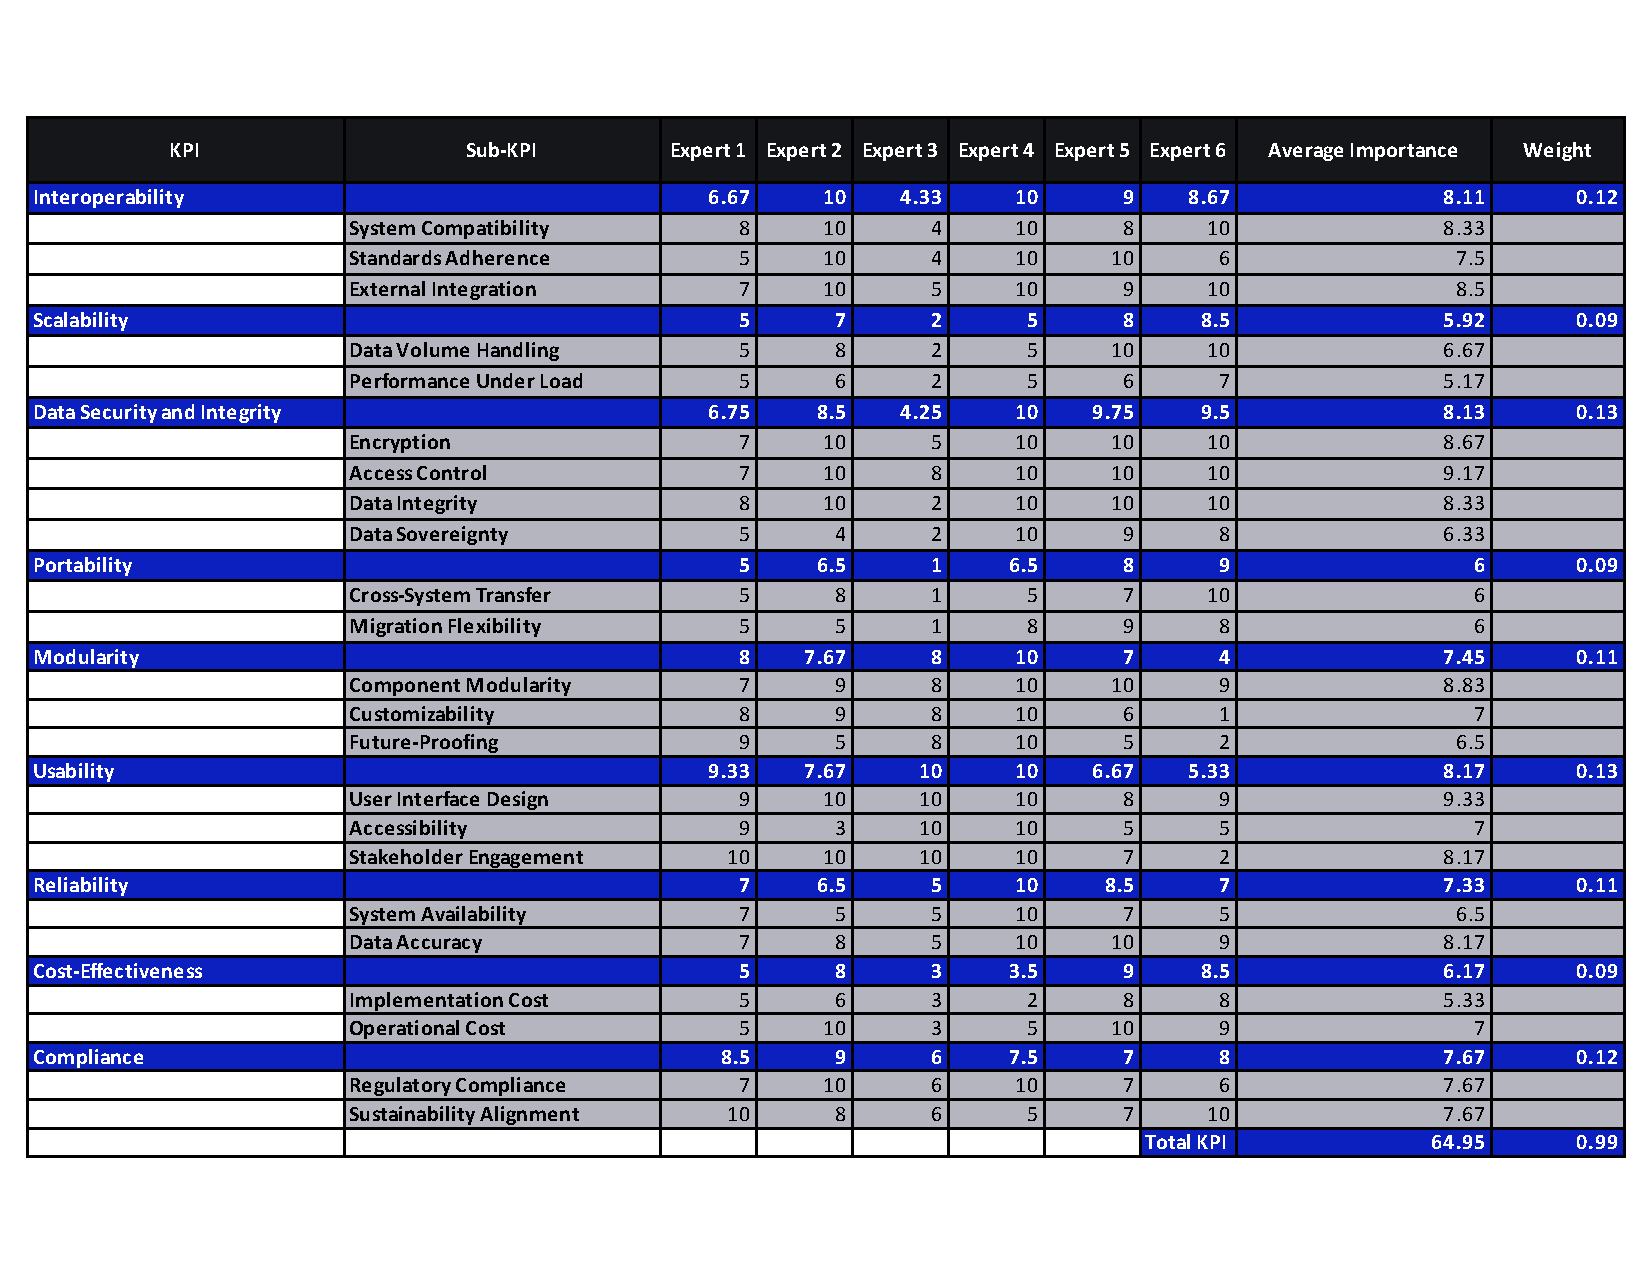
\includegraphics[width=\textwidth]{figures/expert_kpi_calculations.pdf}
  \caption{%
    \textit{\ac{kpi} Weight Calculations} 
  }
  \label{fig:expert_kpi_calculations}
\end{figure}

This structured methodology, built upon \ac{maut} and the additive weighting approach, provides a transparent and replicable method for systematically aggregating expert judgments into a coherent evaluation framework. Using expert judgments to assign criteria weights provides strong contextual validity. Importantly, the additive weighting model ensures a straightforward interpretability, so that decision-makers clearly understand each criterion's relative weight on final decisions. \autocite{Keeney.1979, Belton.2002, Hwang.1981, Triantaphyllou.2000}


\section{Derivation of a Generic DPP System Design Framework}
\label{sec:generic_system_design_model}

The implementation of \acrlong{dpp} systems, as demonstrated throughout this thesis, embodies a highly complex, multidisciplinary challenge. \ac{dpp} solutions need to address diverse technological requirements, satisfy regulatory standards, and remain adaptable to the varied and continuously evolving demands of different industries and stakeholders. Consequently, designing a unified \ac{dpp} framework that is both flexible and comprehensive requires systematically combining multiple dimensions, from technical aspects such as data storage and interoperability mechanisms, to operational considerations such as governance structures and compliance strategies.

\subsection{Methodology}

To address such complex system design challenges, one of the most prevalent and accepted methodologies is the \ac{gma}, also known as the morphological box approach. Developed by astrophysicist \textcite{Zwicky.1969}, \ac{gma} is a method for systematically structuring and analyzing complex problems characterized by multiple interdependent dimensions. It facilitates a rigorous exploration of possible solutions by breaking down a complex problem into its constituent components, or attributes, and then systematically exploring all possible combinations to arrive at innovative, compatible, and robust system designs. Given the multi-dimensional and cross-sectoral nature of \ac{dpp} systems, \ac{gma} is particularly suitable for generating a generic, modular, and scalable framework. \autocite{Zwicky.1969, Ritchey.2011}

\textcite{Ritchey.2011} particularly emphasizes its value in addressing what he describes as "wicked problems", problems that are ill-defined, involving multiple stakeholders, and lacking clear solution pathways. The development of a generic \ac{dpp} system design is such a "wicked" problem, given the heterogeneous technological possibilities, stakeholder diversity, and regulatory fluidity illustrated throughout \Cref{cha:chapter_2,cha:chapter_3}. Morphological analysis is operationalized through the morphological box (or morphological field) methodology. This morphological box method consists of explicitly defined methodological steps, each adapted and followed within this thesis to derive the generic \ac{dpp} design framework \autocite{Ritchey.2011}.

\begin{enumerate}[itemsep=0.5\baselineskip]
    \item[\textbf{Step 1:}] ~\textbf{Definition of Problem and Objective}\\
    The first step involves clearly defining the specific design or decision-making problem and explicitly articulating the overall objectives of the morphological analysis. \autocite[12]{Ritchey.2011}

    \item[\textbf{Step 2:}] ~\textbf{Identification of Key Dimensions (Attributes)}\\
    The defined problem is then systematically decomposed into its constituent attributes or dimensions representing critical aspects of the technological, operational, or regulatory context. \autocite[12]{Ritchey.2011}

    \item[\textbf{Step 3:}] ~\textbf{Defining Options per Dimension}\\
    Each dimension is subsequently described through specific, realistic options or states, each representing discrete alternatives validated by empirical findings, expert evaluations, or literature-derived evidence. \autocites[][12]{Ritchey.2011}[][]{Ritchey.2015}

    \item[\textbf{Step 4:}] ~\textbf{Constructing the Morphological Box}\\
    The dimensions and corresponding options are comprehensively arranged within a morphological box. This combinatorial matrix defines the complete theoretical solution space, wherein each row represents a distinct dimension, and columns correspond to discrete viable alternatives. Initially, no options are excluded, enabling comprehensive representation of the problem space. \autocite[12]{Ritchey.2011}

    \item[\textbf{Step 5:}] ~\textbf{Evaluating and Discarding Incompatible Combinations}\\
    After constructing the morphological box, the compatibility among options across dimensions is systematically assessed. At this stage, unrealistic, impractical, or conflicting combinations are discarded based on logical reasoning, empirical insights, or expert judgments. The outcome is a manageable set of internally consistent and viable system configurations. \autocites[][13]{Ritchey.2011}[][]{Ritchey.2015}

    \item[\textbf{Step 6:}] ~\textbf{Deriving the Generic Model}\\
    The consistent solutions derived from the previous step are synthesized into a generic or representative model. This synthesis integrates the most promising and broadly applicable attribute combinations into a generic model, which serves as a structured conceptual laboratory, facilitating structured exploration of system configurations. \autocites[][14]{Ritchey.2011}[][]{Ritchey.2015}
\end{enumerate}

Fundamentally, \ac{gma} is iterative in nature, employing successive cycles of analysis and synthesis to progressively refine both the problem definition and its solution space. \autocite{Ritchey.2011, Ritchey.2015}

Additionally, the morphological approach strongly encourages and benefits from facilitated group processes involving field experts and various stakeholders, in order to integrate various different perspectives and expertise areas into the final morphological model \autocite[64--68]{Ritchey.2011}. For this reason, this thesis explicitly integrates expert insights and industry perspectives captured in \Cref{sec:expert_insights_evaluation}.

\subsection{Application}

\textbf{Step 1: Definition of Problem and Objective}

As previously established by \textbf{RQ1}, the primary research objective of this thesis is to identify the core technological solutions and frameworks available for developing \ac{dpp} systems and describing them in a generic \ac{dpp} system design model. Thus, the morphological analysis will be aimed at describing the viable technological configurations available for such systems.

\textbf{Step 2: Identification of Key Dimensions (Attributes)}

The systematic identification of key dimensions for this step of the analysis has already been conducted in \Cref{cha:chapter_2}, \Cref{cha:chapter_3} and \Cref{sec:expert_insights_evaluation} of \Cref{cha:chapter_4} through comprehensive literature review, data analysis of existing industry initiatives, and expert interviews respectively.

According to the research findings, the following dimensions represent analytically distinct aspects crucial for the comprehensive system design of a \ac{dpp} system:

\begin{itemize}
    \item \textbf{Data Storage Model}: Determines the approach to data distribution, ownership and hosting, as outlined in \Cref{sec:dpp_concept_architecture} and evaluated empirically in \Cref{sec:data_analysis}.

    \item \textbf{Storage Solution}: Captures the specific technology for data persistence.

    \item \textbf{Ledger Technology}: Whether a decentralized ledger is present in the system design and what type of immutable ledger/\ac{dlt} is implemented.

    \item \textbf{Data Model}: Defines the logical schema (e.g., JSON document, relational table, graph) used to structure passport data.

    \item \textbf{Governance Structure}: Describes who controls data creation, modification, and audit (central authority, service providers, self-sovereign).

    \item \textbf{Digital Twin}: Determines whether the system implements a structured digital representation of products, a key technological enabler discussed thoroughly in \Cref{sec:technology_review}.

    \item \textbf{Semantic Model}: Identifies the explicit semantic standards used for field definitions and relationships, such as the \ac{aas} or UNTP-based schemas, elaborated in \Cref{sec:technology_review,sec:regulatory_landscape}.

    \item \textbf{Resolver Architecture}: Specifies how product identifiers are resolved to their data endpoints, explored in ZVEI's and CIRPASS's architectures in \Cref{sec:dpp_concept_architecture}.

    \item \textbf{Regulatory Scope}: Captures the specific regulatory frameworks the \ac{dpp} system must comply with, explicitly examined in the regulatory analysis of  \Cref{sec:regulatory_landscape}.

    \item \textbf{Authentication}: Defines how actors prove identity (centralized vs. decentralized).

    \item \textbf{Access Control}: Characterizes mechanisms for managing user permissions and data access rights.

    \item \textbf{Data Exchange Protocol}: Specifies the standardized methods and protocols for data interchange between stakeholders.

    \item \textbf{Data Query Protocol}: Defines how consumers query passport data through the specified data exchange protocol.

    \item \textbf{Data Update Pattern}: Describes the method, frequency and dynamicity of updates to product information.

    \item \textbf{Lifecycle Coverage}: Determines which product lifecycle stages are tracked.

    \item \textbf{Security and Trust}: Specifies cryptographic and privacy measures used to ensure data integrity and confidentiality.

    \item \textbf{Scalability Infrastructure}: Addresses the technological framework responsible for the system’s continuous adaptability to increased data volume and user demand.
    
    \item \textbf{AI Integration}: Flags whether \ac{ai} components are present in the system to consume or enrich passport data, discussed as complementary enabling technologies in \Cref{sec:technology_review}.

    \item \textbf{Data Carrier Technology}: Selects the physical data carrier for storing the \ac{dpp} identifier on the physical product. The available options are thoroughly compared in \Cref{sec:dpp_concept_architecture}.

    \item \textbf{User Interaction Layer}: Designates the the front‑end interface(s) provided to stakeholders, as part of the The User and Application Layer introduced in \Cref{sec:dpp_concept_architecture}.
\end{itemize}

\textbf{Step 3 and Step 4: Defining Options per Dimension and Constructing the Morphological Box}

In Step 3, specific, realistic, and viable technological and architectural options were defined for each dimension based on thorough research. 

\begin{table}[!hb]
    \centering
    \caption{Morphological Box of Technological and Architectural Options for DPP Systems}
    \renewcommand{\arraystretch}{1.2}
    \small
    \setlength{\emergencystretch}{3em}
    \begin{tabularx}{\linewidth}{|>{\centering\arraybackslash}m{3.5cm}|*{4}{>{\centering\arraybackslash}X|}}
        \hline
        \cellcolor{myDarkBlue}\textcolor{white}{\textbf{Dimension}} &
        \multicolumn{4}{c|}{\cellcolor{myDarkBlue}\textcolor{white}{\textbf{Options}}} \\
        \hline

        \cellcolor{myGrey}\textbf{Data Storage Model} & Centralized & Federated & Decentralized & -- \\ \hline

        \cellcolor{myGrey}\textbf{Storage Solution} & Relational DB & Document DB & Graph DB & Distributed Ledger \\ \hline

        \cellcolor{myGrey}\textbf{Ledger Technology} & None & Permissioned Blockchain & Permissionless Blockchain & DAG based \ac{dlt} \\ \hline

        \cellcolor{myGrey}\textbf{Data Model} & Relational Schema & JSON Document & Knowledge Graph & -- \\ \hline

        \cellcolor{myGrey}\textbf{Governance Structure} & Central Authority & Service Providers & Self Sovereign & -- \\ \hline
        
        \cellcolor{myGrey}\textbf{Digital Twin} & Yes & No & -- & -- \\ \hline

        \cellcolor{myGrey}\textbf{Semantic Model} & \ac{aas} Schema & UNTP Schema & Proprietary Schema & -- \\ \hline

        \cellcolor{myGrey}\textbf{Resolver Architecture} & None & Single Resolver & Tiered Resolver & Distributed Resolver \\ \hline

        \cellcolor{myGrey}\textbf{Regulatory Scope} & \ac{espr} & Sector-specific & Global  & -- \\ \hline

        \cellcolor{myGrey}\textbf{Authentication} & Centralized IAM & Decentralized \ac{did} & -- & -- \\ \hline

        \cellcolor{myGrey}\textbf{Access Control} & \ac{rbac} & ABAC & Smart Contracts & -- \\ \hline

        \cellcolor{myGrey}\textbf{Data Exchange Protocol} & REST \ac{api} & GraphQL & Event driven & Proprietary \\ \hline

        \cellcolor{myGrey}\textbf{Data Query Protocol} & None & GraphQL & SPARQL & -- \\ \hline

        \cellcolor{myGrey}\textbf{Data Update Pattern} & Batch & Event-driven & Real-time & -- \\ \hline

        \cellcolor{myGrey}\textbf{Lifecycle Coverage} & Cradle-to-Gate & Full Lifecycle & End-of-Life Only & -- \\ \hline

        \cellcolor{myGrey}\textbf{Security \& Trust} & Standard Cryptography & Verifiable Credentials & PETs & -- \\ \hline

        \cellcolor{myGrey}\textbf{Scalability Infrastructure} & Cloud-native & Edge Computing & Blockchain Scalability & -- \\ \hline

        \cellcolor{myGrey}\textbf{AI Integration} & AI Components Integrated & No AI Integration & -- & -- \\ \hline

        \cellcolor{myGrey}\textbf{Data Carrier Technology} & \ac{qr} Code & \ac{rfid} & \ac{nfc} & Other \\ \hline

        \cellcolor{myGrey}\textbf{User Interaction Layer} & Mobile Application & Web Application & \ac{api} only & -- \\ \hline
    \end{tabularx}
    \label{tab:morphological_box_dpp}
\end{table}

In Step 4, these options were then organised into a structured morphological box that maps the analytically defined system design space of possible \ac{dpp} solutions; the fully populated box is presented in \Cref{tab:morphological_box_dpp}.

\textbf{Step 5: Evaluating Cross-Consistency and Discarding Incompatible Combinations}

Following the construction of the morphological box, this step involves conducting a structured Cross-Consistency Assessment (CCA) to explicitly evaluate and exclude logically incompatible or practically infeasible option combinations \autocite[13]{Ritchey.2011}. The criteria for incompatibility were established through logical reasoning, insights from theoretical foundations (\Cref{cha:chapter_2}), empirical observations of industry practice (\Cref{cha:chapter_3}), and expert evaluations (\Cref{sec:expert_insights_evaluation}). The explicit compatibility criteria applied in this assessment are structured below.

\begin{enumerate}[itemsep=0.5\baselineskip]
    \item[\textbf{Criterion 1:}] ~\textbf{Decentralization vs. Centralization Consistency}\\
    This criterion captures logical dependencies related to the decentralization or centralization of system components. Decentralized solutions inherently require congruent decentralized governance and identity structures. Similarly, centralized approaches necessitate corresponding centralized structures.

    \textbf{Incompatible combinations:}
    \begin{itemize}
        \item Decentralized Data Storage Model \textbf{~is incompatible with~} Central Authority Governance.
        \item Centralized Data Storage Model \textbf{~is incompatible with~} Self-Sovereign Governance, Distributed Resolver Architecture, Blockchain Scalability.
        \item Permissionless Blockchain or DAG-based \ac{dlt} \textbf{~is incompatible with~} Central Authority Governance, Centralized IAM Authentication.
        \item Verifiable Credentials \textbf{~is incompatible with~} Centralized IAM Authentication.
    \end{itemize}
    
    Notably, permissioned blockchains can support both centralized and decentralized authentication schemes. 

    \item[\textbf{Criterion 2:}] ~\textbf{Storage Solution and Data Model Compatibility}\\
    Certain storage solutions inherently limit or determine compatible data model options due to underlying technological architecture.
    
    \textbf{Incompatible combinations:}
    \begin{itemize}
        \item Relational Database \textbf{~is incompatible with~} RDF/OWL Knowledge Graph.
        \item Graph Database \textbf{~is incompatible with~} Relational Schema.
        \item Document Database \textbf{~is incompatible with~} RDF/OWL Knowledge Graph.
        \item Distributed Ledger \textbf{~is incompatible with~} Relational Schema.
    \end{itemize}

    \item[\textbf{Criterion 3:}] ~\textbf{Digital Twin and Semantic Model Dependency}\\
    Semantic models explicitly depend on the presence of digital twins, as they provide structured representations of products.
    
    \textbf{Incompatible combinations:}
    \begin{itemize}
        \item Digital Twin option "No" \textbf{~is incompatible with~} \ac{aas} Schema, UNTP Schema, Proprietary Schema.
    \end{itemize}

    \item[\textbf{Criterion 4:}] ~\textbf{Regulatory Scope and Lifecycle Coverage Alignment}\\
    The \ac{espr} explicitly mandates comprehensive product lifecycle coverage for effective circularity and sustainability tracking.
    
    \textbf{Incompatible combinations:}
    \begin{itemize}
        \item \ac{espr} Regulatory Scope \textbf{~is incompatible with~} End-of-Life Only Lifecycle Coverage, Cradle-to-Gate Lifecycle Coverage (without circularity considerations).

    \item[\textbf{Criterion 5:}] ~\textbf{Data Exchange Protocol and Data Query Protocol Alignment}\\
    Certain query protocols require explicit underlying data models or exchange protocols.
    
    \textbf{Incompatible combinations:}
    \begin{itemize}
        \item SPARQL Endpoint \textbf{~is incompatible with~} JSON Document or Relational Schema data models (requires RDF/OWL Knowledge Graph).
        \item Event-driven Data Exchange Protocol \textbf{~is incompatible with~} Data Query Protocol "None" (event-driven data exchange inherently requires querying/subscription mechanisms).
    \end{itemize}
    \end{itemize}
\end{enumerate}

Applying these explicitly defined compatibility criteria systematically excludes infeasible and logically inconsistent combinations from the initial morphological box. While the framework captures general technological and structural incompatibilities, it does not account for additional case‑, industry‑, or regulation‑specific constraints, which must be evaluated separately. Furthermore, depending on system complexity and component granularity, more than one option within a single dimension may be employed in a given architecture. This model is therefore not intended to restrict design choices but to serve as a structured blueprint for the initial conceptualization of \ac{dpp} solutions.

\textbf{Step 6: Deriving the Generic Model}

Following the cross-consistency assessment in Step 5, the solution space defined by the morphological box was systematically reduced to a set of internally coherent and practically viable \ac{dpp} system configurations. Rather than prescribing a single "ideal" solution, this thesis adopts a configurational approach that recognizes the diversity of industry contexts, regulatory requirements, and technological maturity levels.

The resulting generic model is expressed as a decision logic graph in \Cref{fig:dpp_generic_model}, which formalizes the inter-dependencies among architectural choices. It guides the structured narrowing of the design space based on prior decisions, ensuring internal compatibility and architectural integrity. This model does not dictate fixed solutions but enables flexible system synthesis aligned with specific boundary conditions, such as decentralization level, regulatory compliance scope, or integration depth with digital twins. The graph captures key architectural decision paths and their valid continuations, reflecting the configurational diversity empirically identified in the industry dataset and expert interviews. It distinguishes between core architectural elements with logical precedence (e.g., storage model, governance structure, semantic modeling) and peripheral yet essential components (e.g., user interface, data carrier technology), which, while structurally independent, remain integral to full-system implementation.

As such, the generic model serves as a conceptual blueprint for systematically designing \ac{dpp} systems. It provides both a foundation for practical architecture development and a tool for analytical comparison of existing or proposed system implementations.

\begin{figure}[!ht]
  \centering
  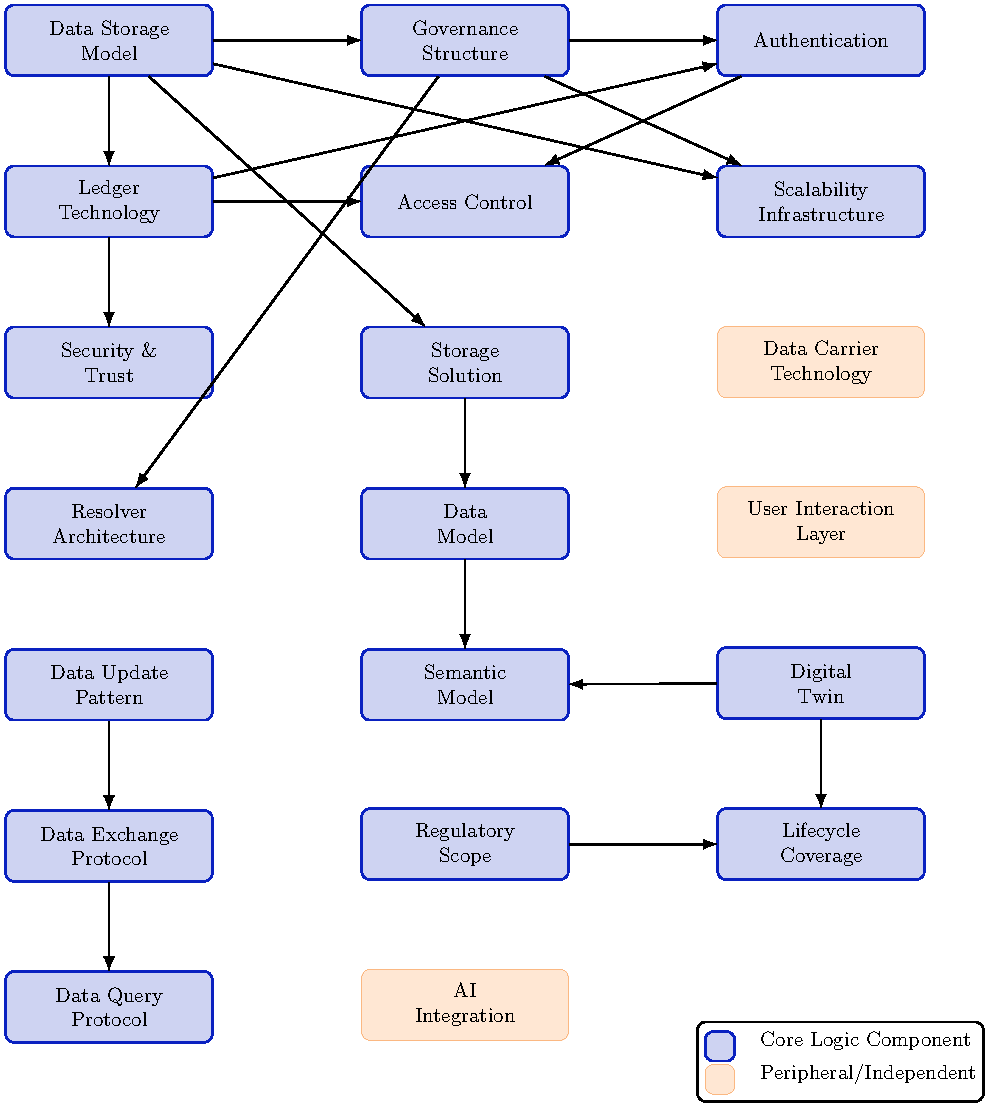
\includegraphics[width=\textwidth]{figures/dpp_generic_model.pdf}
  \caption{%
    \textit{Generic \ac{dpp} System Design as Decision Logic Graph} 
  }
  \label{fig:dpp_generic_model}
\end{figure}
